\chapterimage{QuizCover} % Chapter heading image

\chapter{Pumping Assessment}
% \textbf{Multiple Choice}

\section*{Pumping Assessment}

\begin{enumerate}




\item A 240 volt motor runs an average of 8 hours a day.  If the electric meter registered 6,450 kilowatt hours for a 31-day month, what is the motor horsepower? [35 Hp]




\item A pump is equipped with a pressure gauge in the discharge pipe that reads 100 psi. The total discharge head in feet would be?\\
\vspace{0.4cm}
$100psi*\frac{2.31ft \enspace water}{psi}=\boxed{231ft \enspace water}$
\vspace{0.4cm}

\vspace{0.4cm}
\item 900 GPM pump is pumped against a 12 ft head.  What is the water Hp
\vspace{0.4cm}
water Hp = flow * head\\
$900GPM*12ft*\frac{Hp}{3,960 GPM-ft}=\boxed{2.7Hp}$

\item A 50 ft$^3$/sec flow is pumped against a head of 8 feet.  What is the water Hp

\vspace{0.4cm}
water Hp = flow * head\\
$\dfrac50{ft^3}{sec}*8ft*\frac{7.48 gal}{ft^3}*\frac{60sec}{min}*\frac{Hp}{3,960 GPM-ft}=\boxed{45.4Hp}$

\item 1 MGD is pumped against a 14’ head.  What is the water Hp?  The pump mechanical efficiency is 85\%.  What is the brake horsepower?\\
\vspace{0.4cm}
water Hp = flow * head\\
$\frac{1,000,000gal}{day}*\frac{day}{1440min}*14ft*\frac{Hp}{3,960 GPM-ft}=\boxed{Water \enspace Hp = 2.46Hp}$\\
\vspace{0.4cm}
pump Hp = brake Hp * pump efficiency\\
$brake \enspace Hp = \frac{2.46}{0.85}=\boxed{Brake \enspace Hp=2.89Hp}$


\item A flow of 2.5 MGD is being lifted 10 feet and then pumped up another 120 feet to a storage reservoir. Calculate the pump output power required to lift this water. Ignore friction losses.\\
\vspace{0.4cm}
water Hp = flow * head\\
$\frac{2,500,000gal}{day}*\frac{day}{1440min}*(120+10)ft*\frac{Hp}{3,960 GPM-ft}=\boxed{Water \enspace Hp = 57Hp}$\\
\pagebreak


\item A pump is pumping 400 gpm.  The suction pressure gauge indicates a pressure of 5 ft and the pump discharge pressure gauge indicates a pressure of 100 ft.  If the pump brake horse power is 12 hp, what is the pump efficiency\\
\vspace{0.4cm}
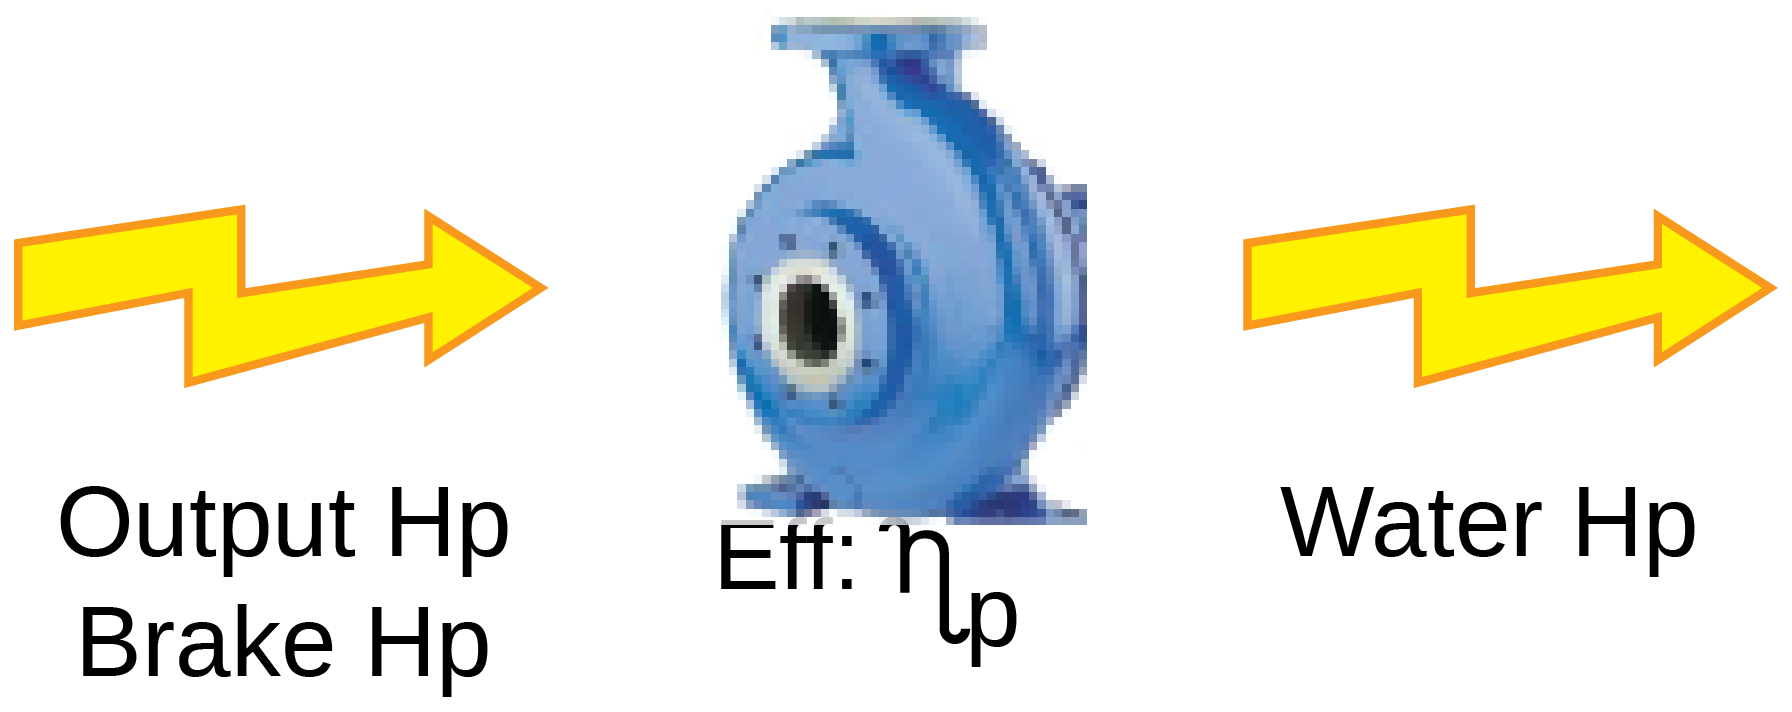
\includegraphics[scale=0.08]{PumpProblemPumpHp}\\
water Hp = flow * head\\
$400gpm*(100-5)ft*\frac{Hp}{3,960 gpm-ft}=\boxed{9.6Hp}$\\
\vspace{0.4cm}
pump efficiency - $\eta_p$=$\frac{9.6Hp}{12Hp}*100=\boxed{79\%}$
\vspace{0.4cm}

\item A flow of 200 gpm  is pumped against a total head of 4.0 feet. · The pump is 78\% efficient and the motor' is 90\% efficient. Calculate the input Hp.\\
\vspace{0.4cm}
water Hp = flow * head\\
$200GPM*4ft*\frac{Hp}{3,960 GPM-ft}=0.2Hp$\\
\vspace{0.4cm}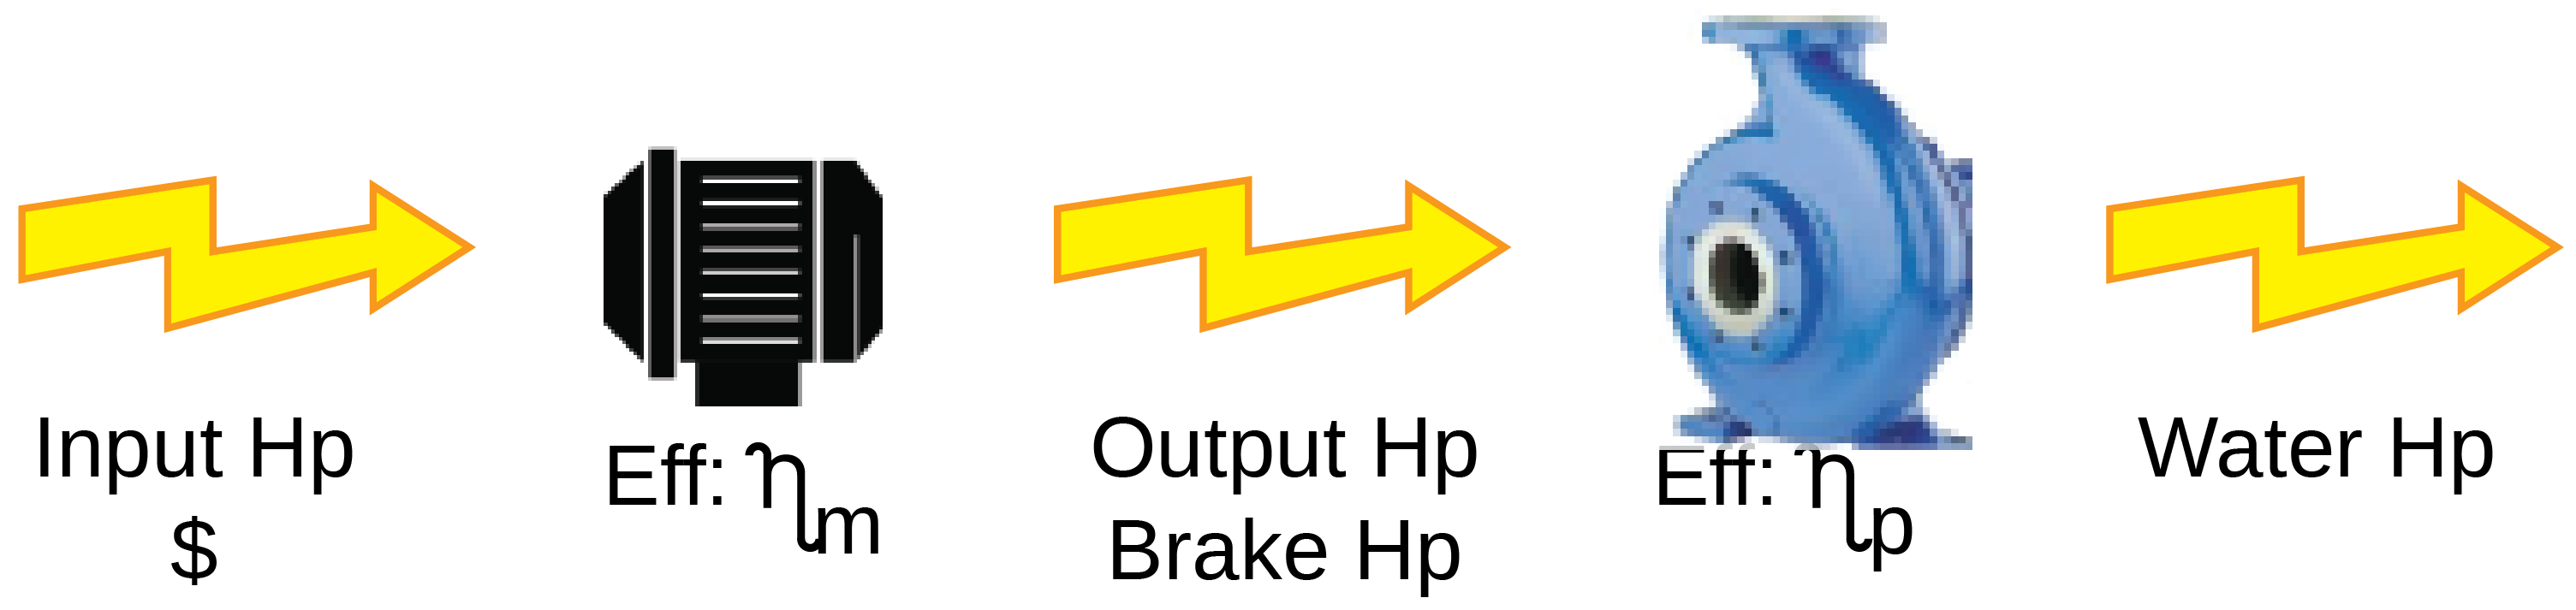
\includegraphics[scale=0.08]{PumpProblem}\\
water Hp=brake Hp*pump efficiency, and\\
brake Hp=input Hp*motor efficiency\\
Therefore, water Hp=input Hp*motor efficiency*pump efficiency\\
\vspace{0.4cm}
input Hp=$\frac{water \enspace Hp}{motor \enspace efficiency*pump \enspace efficiency}=\frac{0.2}{0.9*0.78}=\boxed{0.28Hp}$

\pagebreak

\item 500,000 gpd of secondary· effluent is pumped to  a  storage  pond  for  reuse  as golf course irrigation water.  The water is lifted 12 feet in the plant, and then pumped up another 75 feet to the storage pond. Friction losses are assumed to be 10\% of the static head.  Assuming the pump efficiency of 70\% and a motor efficiency of 92\% and an electrical cost of \$0.0725 per KWh, calculate the daily cost of pumping this water.\\
\vspace{0.4cm}
Solution:\\

water Hp = flow * head\\
\vspace{0.4cm}
$\frac{500,000gal}{day}*\frac{day}{1440min}*(87ft-static \enspace head+87*0.1ft-friction \enspace head)*\frac{Hp}{3,960 GPM-ft}$\\
$=8.39 - water \enspace Hp$\\
\vspace{0.4cm}
input Hp=$\frac{water \enspace Hp}{motor \enspace efficiency*pump \enspace efficiency}=\frac{8.39}{0.92*0.70}=\boxed{13Hp}$\\
\vspace{0.4cm}
Electrical cost=$13Hp*\frac{0.746kW}{Hp}*\frac{24hrs}{day}*\frac{\$0.0725}{kWh}=\boxed{\frac{\$16.87}{day}}$

\vspace{0.4cm}


\item A pump motor (93\% efficient) generates an output of 130 HP and runs 75\% of the time. Electricity costs an average of 8.455 cents per kilowatt-hour. What is the monthly cost of operating this pump in \$ per month?\\
\vspace{0.4cm}
$\frac{130Hp}{0.93}*\frac{0.746kW}{Hp}*\frac{24hrs}{day}*\frac{30days}{month}*0.75*\frac{\$0.08455}{kWh}=\boxed{\frac{\$4,761}{month}}$
\pagebreak


\item A wet well is 8 ft x 8 ft x 16.5 ft deep and receives a continuous flow of 310,000 gpd.  A 500 gpm pump draws down 12 feet of water each pumping cycle.  The motor that drives the pump draws 52.5 Hp when it pumps.  The cost of electricity is \$0.0755 per kilowatt - hour.  Calculate\\ 
(a) the time it takes to pump down the wet well, and\\
(b) The daily electrical energy cost for this pump.\\


\vspace{0.4cm}
Solution:\\
@$\frac{310,000gal}{day}*\frac{day}{1440min}=\frac{215.3gal}{min}$\\
\vspace{0.4cm}
Volume of wetwell that will be pumped down with the 500 gpm pump and a 215.3 gpm flow to the wetwell:\\
$\frac{500gal}{min}-\frac{215.3gal}{min}=\frac{284.7gal}{min}$\\
\vspace{0.4cm}
Minutes required to pump down the wetwell :\\
$8*8*12ft^3*\frac{7.48gal}{ft^3}*\frac{min}{284.7gal}=\boxed{20.2min}$\\
\vspace{0.4cm}
Time to fill wetwell with pump off @215.3gal/min influent flow:
\\
$8*8*12ft^3*\frac{7.48gal}{ft^3}*\frac{min}{215.3gal}=26.7min$\\
\vspace{0.4cm}
\# of cycles per day:\\
$\frac{cycle}{(20.2+26.7)min}*\frac{1440min}{day}=\frac{30.7cycles}{day}$\\
\vspace{0.4cm}
\# of hrs pump operational:\\
$\frac{20.2min}{cycle}*\frac{30.7 cycles}{day}*\frac{hrs}{60min}=\frac{10.33hours}{day}$\\
\vspace{0.4cm}
Daily electrical cost:\\
$52.5Hp*\frac{0.746kW}{Hp}*\frac{10.33hrs}{day}*\frac{\$0.0755}{kWh}=\boxed{\frac{\$30.54}{day}}$\\
\pagebreak


\item A 6-year old pump motor is to be replaced at a net cost of \$15,800. The new motor, just like the old one, would run 65\% of the time. Both existing and replacement motors would operate at 125 output Hp. The existing motor efficiency is 86\% while the replacement motor would be guaranteed at 94\% efficiency. Electricity currently averages \$0.088 per kWh.\\
(a) Calculate the energy cost savings per year (to the nearest dollar) if the existing motor is replaced with the new motor (neglect any consideration of impact upon demand charges or interest on capital).\\ (b) What is payback period to the nearest tenth of a year.
\vspace{0.4cm}
Energy cost savings per year:\\
Input Hp for old motor:$\frac{125}{0.86}=145.35Hp$\\
Input Hp for old motor:$\frac{125}{0.94}=132.98Hp$\\
Energy cost savings:\\$(145.35-132.98)Hp*\frac{0.746kW}{Hp}*\frac{(365*24*0.65)hrs}{yr}*\frac{\$0.088}{kWh}=\boxed{\frac{\$4,623.94}{yr}}$\\
\vspace{0.4cm}
Calculate payback:\\
$\$15,800*\frac{yr}{\$4,623.94}=\boxed{3.4yr}$

\item A 8 ft diameter cylindrical wetwell receives an average incoming flow if 135 gpm and is pumped down with a pump that delivers 450 gpm again a total dynamic head of 120 ft.  The pump is controlled using two floats; a stop float located at 2.5 ft and a start float located at 16 ft.  If the pump motor is rated at 88\% and the pump at 77\%, what is the monthly (30 days/month) for running this pump if power costs are \$0.11/Kwh? (Ans:  \$356/month)


\vspace{0.4cm}
Volume of wetwell that will be pumped down with the 450 gpm pump and a 135 gpm flow to the wetwell:\\
$\frac{450gal}{min}-\frac{135gal}{min}=\frac{315gal}{min}$\\
\vspace{0.4cm}
Minutes required to pump down the wetwell :\\
$0.785*8^2*(16-2.5)ft^3*\frac{7.48gal}{ft^3}*\frac{min}{315gal}=\boxed{16.1min}$\\
\vspace{0.4cm}
Time to fill wetwell with pump off @135gal/min influent flow:
\\
$[0.785*8^2*(16-2.5)]ft^3*\frac{7.48gal}{ft^3}*\frac{min}{135gal}=37.6min$\\
\vspace{0.4cm}
\# of cycles per day:\\
$\frac{cycle}{(16.1+37.6)min}*\frac{1440min}{day}=\frac{26.8cycles}{day}$\\
\vspace{0.4cm}
\# of hrs pump operational:\\
$\frac{16.1min}{cycle}*\frac{26.8 cycles}{day}*\frac{hrs}{60min}=\frac{7.19hours}{day}$\\
\vspace{0.4cm}
Daily electrical cost:\\
$\frac{450gpm*120ft}{0.88*0.77}*\frac{Hp}{3,960 gpm-ft}*\frac{0.746kW}{Hp}*\frac{7.19hrs}{day}*\frac{30days}{month}*\frac{\$0.11}{kWh}=\boxed{\frac{\$356}{day}}$\\
\vspace{1cm}


\item A pump operating at 80\% effieciency generates an water Hp of 60 HP and runs 75\% of the time. Assuming the pump motor is 90\% efficent and electricity costs an average of \$0.0821 per kilowatt-hour. The monthly (30 days) cost of operating this pump is:\\
\vspace{0.4cm}
$\frac{60Hp}{0.90*0.80}*\frac{0.746kW}{Hp}*\frac{24hrs}{day}*\frac{30days}{month}*0.75*\frac{\$0.0821}{kWh}=\boxed{\frac{\$2,756}{month}} - Correct \enspace Answer$\\
$\frac{60Hp}{0.8}*\frac{0.746kW}{Hp}*\frac{24hrs}{day}*\frac{30days}{month}*0.75*\frac{\$0.0821}{kWh}=\boxed{\frac{\$2,480}{month}}$\\
$\frac{60Hp}{0.90}*\frac{0.746kW}{Hp}*\frac{24hrs}{day}*\frac{30days}{month}*0.75*\frac{\$0.0821}{kWh}=\boxed{\frac{\$2,205}{month}}$\\
$\frac{60Hp}{0.90*0.80}*\frac{0.746kW}{Hp}*\frac{24hrs}{day}*\frac{30days}{month}*\frac{\$0.0821}{kWh}=\boxed{\frac{\$3,675}{month}}$

\item A 8 ft diameter cylindrical wetwell receives an average incoming flow if 135 gpm and is pumped down with a pump that delivers 450 gpm again a total dynamic head of 120 ft. The pump is controlled using two floats; a stop float located at 2.5 ft and a start float located at 16 ft. If the pump motor is rated at 88\% and the pump at 77\%, what is the monthly (30 days/month) for running this pump if power costs are \$0.11/Kwh? (Ans: \$356/month) 

\item  A 8 ft diameter cylindrical wetwell receives an average incoming flow if 135 gpm and is pumped down with a pump that delivers 450 gpm again a total dynamic head of 120 ft. The pump is controlled using two floats; a stop float located at 2.5 ft and a start float located at 16 ft. If the pump motor is rated at 88\% and the pump at 77\%, what is the monthly (30 days/month) for running this pump if power costs are \$0.11/Kwh? (Ans: \$356/month)


\item If a wasting pump has a fixed pump rate of 250 GPM, and your calculation
indicates you must waste 126,000 gallons, what hourly cycle rate do you set
the timer?\\
a. Turn pump on 21 minutes every day\\
b. Turn pump on 504 minutes every hour\\
c. Turn pump on 42 minutes every day\\
d. Turn pump on 21 minutes every hour\\

\vspace{0.3cm}
Solution:\\
\vspace{0.2cm}
$\frac{min}{hr}=\frac{126,000 \enspace gal}{day}*\frac{day}{24 \enspace hrs}*\frac{min}{250 \enspace gal}=\boxed{\frac{21 \enspace min}{hr}}$



\item  How long will it take to pump down 25 feet of water in a 110 ft diameter cylindrical tank when using a 1420 gpm pump. 

a. 26 hours and 56 minutes \\
*b. 26 hours and 33 minutes \\
c. 2 hours and 47 minutes \\
d. 12 hours and 36 minutes 


\item  A positive displacement pump should be started up with the discharge valve closed in order to avoid any problems with "air lock". 

a. True \\
*b. False 


\item  Brake horse power is the input power to the motor 

a. True \\
*b. False 


\item  Cost of electrical usage for pumps is based upon kilowatt per hour 

a. True \\
*b. False 


\item  A centrifugal pump can be used to pump sludge. 

*a. True \\
b. False 


\item  Variable speed sludge pumps may be used to keep the density of the sludge nearly constant. 

*a. True \\
b. False

\item The keeping of records of plant operation and maintenance, even when a portion of the plant is temporarily out of balance, is an integral part of good operation.\\
*a. True\\
b. False 


\item  A positive displacement pump could be damaged if it is started with the discharge valve closed. \\

*a. True \\
b. False 


\item  The common unit of power or rate of doing work is horsepower. This· is equal to 746 ft. lbs/min. 

*a. True \\
b. False 


\item  Total dynamic head is the sum of the suction head and the discharge head minus the friction head 

a. True \\
*b. False 


\item  Water power is the output power of the pump 

*a. True \\
b. False 


\item  A positive displacement pump should be started up with the discharge valve closed in order to avoid any problems with "air lock". 

a. True \\
*b. False 


\item  Brake horse power is the input power to the motor 

a. True \\
*b. False 


\item  Cost of electrical usage for pumps is based upon kilowatt per hour 

a. True \\
*b. False 


\item  The common unit of power or rate of doing work is horsepower. This· is equal to 746 ft. lbs/min. 

*a. True \\
b. False 


\item  Total dynamic head is the sum of the suction head and the discharge head minus the friction head 

a. True \\
*b. False 


\item  Water power is the output power of the pump 

*a. True \\
b. False 

\item  What is the vertical distance between the elevation of the free water surface at the suction and that of the free water surface at the discharge of a pump called?\\
a.	Discharge head.\\
b.	Dynamic head.\\
c.	Velocity head.\\
*d.	Static head.\\

\item If a wasting pump has a fixed pump rate of 250 GPM, and your calculation
indicates you must waste 126,000 gallons, what hourly cycle rate do you set
the timer?\\
a. Turn pump on 21 minutes every day\\
b. Turn pump on 504 minutes every hour\\
c. Turn pump on 42 minutes every day\\
*d. Turn pump on 21 minutes every hour\\

\item A positive displacement pump is connected to a 25' wide x 125' long x 12' side water depth aerobic digester. How long will it take to empty the contents of the digester if the pump rate is 225 gallons per minute?\\
a. 15.3 hours\\
b. 2.8 hours\\
*c. 20.8 hours\\
d. 15.6 hours\\

\item A centrifuge is fed sludge with a concentration of 3.4\% solids. If the sludge feed rate is set at 50 gallons per minute, what is the centrifuge loading rate
in pounds per hour?\\
a. 763 lbs/hour\\
*b. 850 lbs/hour\\
c. 735 lbs/hour\\
d. 960 lbs/hour\\

\item Calculate the surface loading rate for a treatment plant with 4 clarifiers each
with a 100 foot diameter. The plant has an influent flow of 35 MGD.\\
a. 279 gal/sq ft\\
b. 950 gal/sq ft\\
c. 4,459 gal/sq ft\\
*d. 1,115 gal/sq ft\\

\item Calculate the flow velocity in feet/minute if 7.5 MGD of flow passes through a channel that is 3' wide x 4' deep, and the depth of flow is 15 inches.\\
*a. 186 ft/min\\
b. 58 ft/min\\
c. 202 ft/min\\
d. 46.5 ft/min\\

\item Determine the pounds per day of primary solids removed at a plant with a flow rate of 1.5 MGD and the following data:\\
Clear Waters Fall 2013\\
Influent TSS = 250 mg/L\\
Primary Effluent TSS = 150 mg/L,\\
Final Effluent TSS = 12 mg/L\\
a. 1,101 lbs/day\\
*b. 1,251 lbs/day\\
c. 982 lbs/day\\
d. 2,977 lbs/day\\

\item A sewage pump is located above the wet well which is 8 feet deep and the
pump is pumping to an above ground clarifier with 12 feet depth of water.
The pump manufacturer has given you the pump characteristics curve
which shows Total Dynamic Head vs. flow rates. If the operating wet well
water depth is 6 feet, what is the total dynamic head in order to determine
pumping rate from the chart? Assume the top of the wet well and the
bottom of the clarifier are at the same elevation.\\
a. 12 feet\\
b. 20 feet\\
*c. 14 feet\\
d. 10 feet\\

\item A sewage pump is located above the 8-foot diameter wet well which is
8 feet deep and the pump is pumping to an above ground clarifier. The flow
meter on the pump is not operating and you want to calculate the pumping
rate by measuring the drop in wet well water level during when inflow to
wet well is minimal? If the drop in water level in one minute is 2 feet, what
is the approximate pumping rate in gallons per minute?\\
a. 250 GPM\\
b. 375 GPM\\
c. 500 GPM\\
*d. 750 GPM\\

\item The head against which a pump must operate:\\
a. Is the sum of the static head and the head due to friction loss.\\
b. Must always be above the shut-off head.\\
c. Is the static head.\\
d. Is the friction head.\\
\item What term describes the condition that exists when the source of the water supply is below the centerline of the pump?\\
a. Pressure head\\
b. Velocity head\\
c. Suction lift\\
d. Total discharge head\\

\item  A pump operating at 80\% efficiency generates an water Hp of 60 HP and runs 75\% of the time. Assuming the pump motor is 90\% efficent and electricity costs an average of \$0.0821 per kWh. The monthly (30 days) cost of operating this pump is:\\

*a. \$2,756 \\
b. \$2,480 \\
c. \$2,205 \\
d. \$3,675 






\end{enumerate}





